%%%%%%%%%%%%%%%%%%%%%%%%%%%%%%%%%%%%%%%%%%%%%%%%%%%%%%%%%%%%%%%%%%
\subsection{Support Vector Machines (\acrshort{svm})}
\label{sec:svm}

\subsubsection{Puntuación de características}
\label{sec:svm1}

Para la técnica de \gls{svm}, también se procede a desarrollar una primera versión de clasificador para poder visualizar la importancia que toman las características en el mismo. En este caso, se trata de la clase \textit{SVC()} \cite{svc} y se inicializa un objeto de la misma con la definición por defecto de un kernel radial o gaussiano (\gls{rbf}), ya que se trabaja con un conjunto de datos no linearmente separables y que resulta complejo de operar si no se aumenta la dimensionalidad del espacio (ver Sección \ref{sec:mlsvm}). 

\vspace{3mm}

Adicionalmente, \textit{SVC()} determina valores por defecto de los hiperparámetros \textit{C} y \textit{gamma}, que hacen referencia respectivamente, a la regularización del modelo y al impacto que produce cada instancia de entrenamiento en el proceso de clasificación. El clasificador se ejecuta, se entrena con el conjunto de datos y, por consiguiente, se le aplican dos métodos de puntuación de características. Cabe destacar que, en esta primera versión del clasificador del \gls{svm}, el proceso de entrenamiento se caracteriza por presentar una duración mucho mayor que con el \gls{rf} --------------.

\vspace{3mm}

\begin{lstlisting}[style=Python, caption={Clasificador SVM por defecto}]
  classifier = SVC(kernel = 'rbf', random_state = 0) #por defecto C=1, gamma='scale' o 'auto'
  classifier.fit(X_train, y_train)
\end{lstlisting}
  
\vspace{3mm}

Por un lado, se estima la importancia de las características a partir de la distancia que tienen hacia los vectores de soporte. En este caso es preciso basarse en los atributos \textit{support\_vectors\_} y \textit{dual\_coef\_}, que proporcionan la información sobre los vectores soporte que se han definido en el \gls{svm} y los multiplicadores de \textit{Lagrange} asociados. El resultado se expone en la Figura \ref{fig:imp3}, en la cual se visualiza cómo las longitudes de las etiquetas origen y destino inciden en la clasificación significativamente, ya que el resto de características tienen puntuaciones mucho más bajas.

\vspace{3mm}

Por otro lado, al igual que se ha expuesto para el \gls{rf} (ver Sección \ref{sec:rf1}), se incluye el análisis a partir del método de la permutación (\textit{permutation\_importance}). En este caso, las longitudes de las etiquetas siguen siendo predominantes, pero las características que hacen referencia a la capacidad y al flujo total de energía resultante de \gls{den2ne} (\textit{abs\_flux}) también presentan valores de puntuaciones a considerar.

\begin{figure}[H]
    \centering
    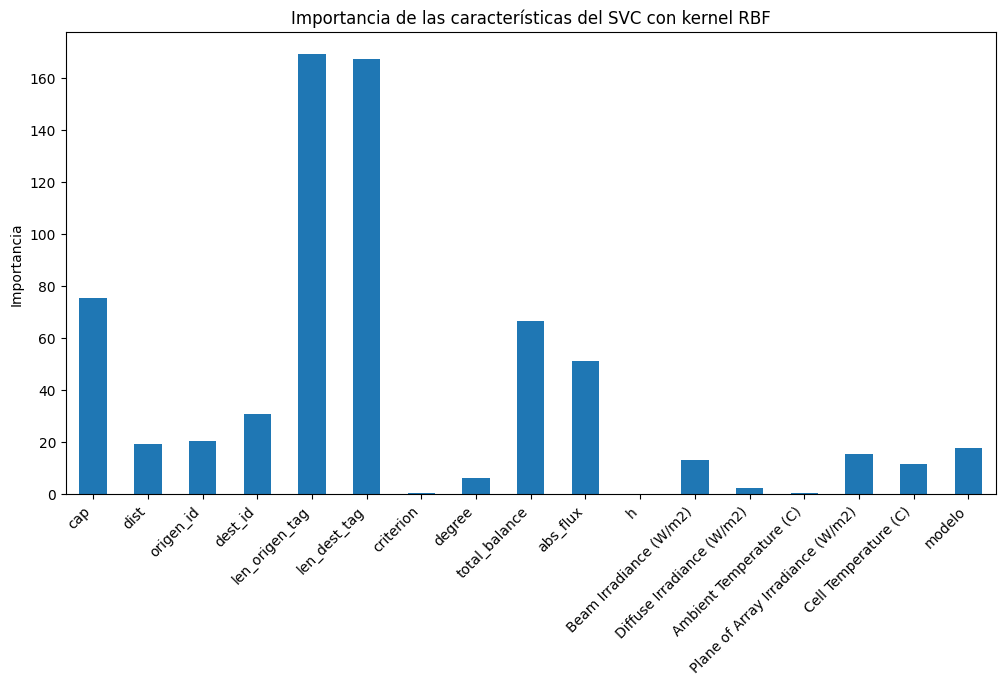
\includegraphics[width=1\textwidth]{img/desarrollo/svm/importance3.png}
    \caption{Puntuación de características del \acrshort{svm} mediante los atributos \textit{support\_vectors\_} y \textit{dual\_coef\_}}
    \label{fig:imp3}
\end{figure}
  
\begin{figure}[H]
    \centering
    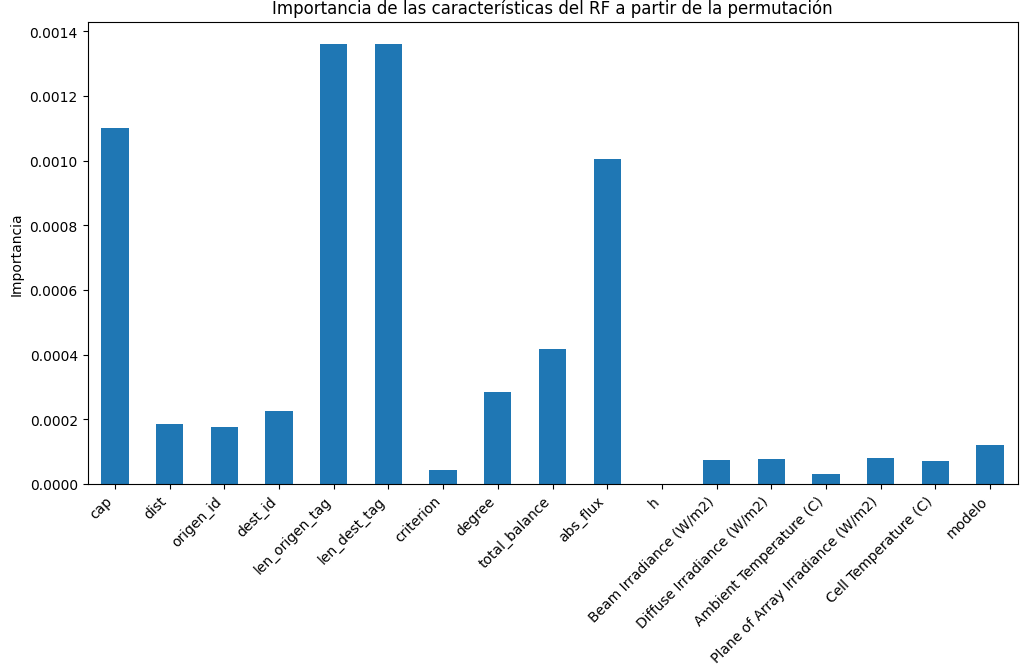
\includegraphics[width=1\textwidth]{img/desarrollo/svm/importance4.png}
    \caption{Puntuación de características del \acrshort{svm} mediante el método \textit{permutation\_importance}}
    \label{fig:imp4}
\end{figure}

\subsubsection{Optimización de hiperparámetros}

Para modelar un \gls{svm} óptimo se centra el estudio en dos hiperparámetros: el tipo de kernel a aplicar y el parámetro de regularización \textit{C}. En el caso de \textit{gamma}, mencionada anteriormente, es indiferente su configuración, puesto que los datos del conjunto han sido previamente escalados (ver Sección \ref{sec:adicional}) y las dos opciones posibles de \textit{gamma} ('scale' o 'auto') solo se diferencian en si se aplica o no la varianza de los datos en el cálculo del parámetro. Por lo tanto, desechando el análisis de \textit{gamma}, se aplica el método \textit{Grid Search} para realizar la búsqueda de la combinación óptima de hiperparámetros.

\vspace{3mm}

\begin{lstlisting}[style=Python, caption={Cuadrícula de parámetros SVM}]
  param_grid = {
    'C': [0.25, 0.5, 0.75, 1], 
    'kernel': ['poly', 'rbf', 'sigmoid']
  }
\end{lstlisting}

\vspace{3mm}

Después, se inicializa un objeto de la clase \textit{GridSearchCV()} y se configura de la misma forma que se detallaba en la Sección \ref{rf2} para el \gls{rf}. No obstante, antes que nada, es importante considerar la duración del entrenamiento de un modelo \gls{svm} a partir del conjunto de datos (ver Sección \ref{sec:svm1}), puesto que es relativamente grande. Por ello, hay que cuantificar cuánto tiempo supone ejecutar todas las combinaciones de hiperaparámetros definidas en el método \textit{Grid Search}, en función del número de procesadores y de los pliegues configurados (\textit{cv=5}). Por tanto, el tiempo total de búsqueda de la combinación óptima se estima en ------------------------.

\vspace{3mm}

La ejecución indica en los atributos \textit{best\_score\_} y \textit{best\_params\_} que el caso óptimo es ------------------------------ con una precisión del ----------------. El análisis detallado de los resultados de rendimiento de todas las combinaciones probadas se proporciona en el atributo \textit{cv\_results\_}, especialmente en el elemento que hace referencia al promedio de precisión obtenida (\textit{mean\_test\_score}) y a los tiempos de entrenamiento (\textit{mean\_fit\_time}). 

%aqui explicar resultados

En la Tabla \ref{tab:svmgs} --------------------------

En la Tabla \ref{tab:svmgs2}  ----------------------

\vspace{3mm}

\begin{table}[H]
  \centering
  \begin{subtable}{0.45\linewidth}
    \centering
    \begin{tabular}{|>{\columncolor[HTML]{EFEFEF}}c |c|c|c|}
      \hline
      \textit{\begin{tabular}[c]{@{}c@{}}Kernel /\\C\end{tabular}} & \cellcolor[HTML]{EFEFEF}\textit{poly} & \cellcolor[HTML]{EFEFEF}\textit{rbf} & \cellcolor[HTML]{EFEFEF}\textit{sigmoid}\\ \hline
      0,25 &  &  & \\ \hline
      0,5 &  &  & \\ \hline
      0,75 &  &  & \\ \hline
      1 &  &  & \\ \hline
    \end{tabular}
    \caption{Precisión (\%) (\textit{mean\_test\_score})}
    \label{tab:svmgs}
  \end{subtable}
  \hfill
  \begin{subtable}{0.45\linewidth}
    \centering
    \begin{tabular}{|>{\columncolor[HTML]{EFEFEF}}c |c|c|c|}
      \hline
      \textit{\begin{tabular}[c]{@{}c@{}}Kernel /\\C\end{tabular}} & \cellcolor[HTML]{EFEFEF}\textit{poly} & \cellcolor[HTML]{EFEFEF}\textit{rbf} & \cellcolor[HTML]{EFEFEF}\textit{sigmoid}\\ \hline
      0,25 &  &  & \\ \hline
      0,5 &  &  & \\ \hline
      0,75 &  &  & \\ \hline
      1 &  &  & \\ \hline
    \end{tabular}
    \caption{Tiempo (s) (\textit{mean\_fit\_time})}
    \label{tab:svmgs2}
  \end{subtable}
  \caption{Resultados extraídos del atributo \textit{cv\_results\_} del \acrshort{svm}}
  \label{tab:svmgs_combined}
\end{table}

\vspace{3mm}



% The parameters of the estimator used to apply these methods are optimized by cross-validated grid-search over a parameter grid.

%  Los hiperparámetros son configuraciones que no se aprenden directamente del proceso de entrenamiento del modelo y que afectan la estructura y el rendimiento del mismo. 

% La optimización de hiperparámetros implica encontrar la combinación óptima de valores para estos hiperparámetros que maximice el rendimiento del modelo en un conjunto de datos dado. Esto puede lograrse mediante técnicas como búsqueda exhaustiva, búsqueda aleatoria, optimización bayesiana o algoritmos de aprendizaje automático basados en modelos (como Grid Search, Random Search, Bayesian Optimization, entre otros).

% Optimizar los hiperparámetros de un Random Forest puede conducir a modelos más precisos, robustos y generalizables. Sin embargo, debido a la complejidad y dimensionalidad del espacio de búsqueda de hiperparámetros, es importante realizar esta optimización de manera eficiente para evitar el sobreajuste y el consumo excesivo de recursos computacionales.



% C a fin de cuentas el hiperparámetro encargado de controlar el balance entre bias y varianza del modelo. En la práctica, su valor óptimo se identifica mediante validación cruzada. Esta es la razón por la que el parámetro  C controla el balance entre bias y varianza lo que permite un ajuste adecuado del modelo. 

%Cuando el valor de  Ces pequeño, el margen es más ancho, y más observaciones violan el margen, convirtiéndose en vectores soporte. El hiperplano está, por lo tanto, sustentado por más observaciones, lo que aumenta el bias pero reduce la varianza. 

%Cuando mayor es el valor de  C , menor el margen, menos observaciones son vectores soporte y el clasificador resultante tiene menor bias pero mayor varianza.

%Otra propiedad importante que deriva de que el hiperplano dependa únicamente de una pequeña proporción de observaciones (vectores soporte), es su robustez frente a observaciones muy alejadas del hiperplano. Esto hace al método de clasificación vector soporte distinto a otros métodos tales como Linear Discrimiant Analysis (LDA), donde la regla de clasificación depende de la media de todas las observaciones.

%%gird search tiempo
%https://datascience.stackexchange.com/questions/29495/how-to-estimate-gridsearchcv-computing-time



\subsubsection{Selección de características}

%hablar del coste computacional
% Reducción de la dimensionalidad: En muchos casos, los conjuntos de datos contienen una gran cantidad de características, algunas de las cuales pueden no contribuir significativamente a la capacidad predictiva del modelo. La selección de características ayuda a reducir la dimensionalidad del espacio de características, lo que puede mejorar la eficiencia computacional y reducir el riesgo de sobreajuste.

% Interpretación y comprensión del modelo: Al seleccionar un subconjunto relevante de características, el modelo resultante puede ser más interpretable y comprensible para los humanos. Esto es especialmente importante en aplicaciones donde se requiere transparencia y explicabilidad del modelo, como en la medicina o el derecho.

% Menor riesgo de sobreajuste: La inclusión de características irrelevantes puede aumentar el riesgo de sobreajuste, donde el modelo se ajusta demasiado a los datos de entrenamiento y tiene un rendimiento deficiente en datos no vistos. La selección de características ayuda a mitigar este riesgo al eliminar características que no contribuyen significativamente a la generalización del modelo.

% Mejora de la eficiencia computacional: Al reducir la dimensionalidad del conjunto de datos, la selección de características puede hacer que el proceso de entrenamiento y predicción sea más rápido y eficiente, lo que es especialmente importante en conjuntos de datos grandes o en entornos con recursos computacionales limitados.

\subsubsection{Ejecución del modelo y evaluación de resultados}






\vspace{3mm}

\begin{table}[H]
  \centering
  \begin{tabular}{|c|c|c|c|c|c|c|c|c|}
  \hline
  \rowcolor[HTML]{EFEFEF} 
  \textit{\begin{tabular}[c]{@{}c@{}}Matriz\\ de confusión\end{tabular}} & \cellcolor[HTML]{EFEFEF}\textit{TN} & \textit{FP} & \textit{FN} & \textit{TP} & \textit{Accuracy} & \textit{Precision} & \textit{Recall} & \textit{F1 Score} \\ \hline
  \cellcolor[HTML]{EFEFEF}\textit{Sin aplicar} &  &  &  &  &  &  &  &  \\ \hline
  \cellcolor[HTML]{EFEFEF}\textit{FS (n=5)} &  &  &  &  &  &  &  &  \\ \hline
  \cellcolor[HTML]{EFEFEF}\textit{FS (n=8)} &  &  &  &  &  &  &  &  \\ \hline
  \cellcolor[HTML]{EFEFEF}\textit{PCA (n=2)} &  &  &  &  &  &  &  &  \\ \hline
  \cellcolor[HTML]{EFEFEF}\textit{PCA (n=4)} &  &  &  &  &  &  &  &  \\ \hline
  \end{tabular}
  \caption{Resultados de aplicación de la matriz de confusión al \gls{svm}}
  \label{tab:rfcm}
\end{table}

\vspace{3mm}





\vspace{3mm}

\begin{table}[H]
  \centering
  \begin{tabular}{|c|c|c|c|c|c|c|c|c|}
  \hline
  \rowcolor[HTML]{EFEFEF} 
  \textit{\begin{tabular}[c]{@{}c@{}}K-Fold\\ Cross Validation\end{tabular}} & \cellcolor[HTML]{EFEFEF}\textit{Accuracy} & \textit{Standard Deviation} \\ \hline
  \cellcolor[HTML]{EFEFEF}\textit{Sin aplicar} &  &  \\ \hline
  \cellcolor[HTML]{EFEFEF}\textit{FS (n=5)} &  &  \\ \hline
  \cellcolor[HTML]{EFEFEF}\textit{FS (n=8)} &  &  \\ \hline
  \cellcolor[HTML]{EFEFEF}\textit{PCA (n=2)} &  &  \\ \hline
  \cellcolor[HTML]{EFEFEF}\textit{PCA (n=4)} &  &  \\ \hline
  \end{tabular}
  \caption{Resultados de aplicación del \textit{K-Fold Cross Validation} al \gls{svm}}
  \label{tab:rfk}
\end{table}